\exercise

Given the directed graph $G$ consisting of nodes $\{A, B, C, D\}$ and edges 
$\{(A,B), (B,C),$ $ (D,C), (C,A)\}$, describe how you compute the similarity
between node $B$ and node $A$ via Personalized PageRank, and then show the
result by iterating it once.

\solution

We observe that the given graph has no sink nodes, so we do not need to add
edges from sink nodes to other nodes. We apply the Personalized PageRank formula
%
\begin{equation*}
  r(i) = \alpha\cdot\sum_{j\in B(i)} \frac{r(j)}{|out(j)|} +
  \begin{cases*}
    1-\alpha & if $i=A$ \\
    0        & otherwise
  \end{cases*},
\end{equation*}
%
where $B(i)$ is the set of nodes linking to $i$, and $out(j)$ is the set of
outgoing links from $j$.

Furthermore, we assume that the initial probability distribution is
$r_0=(1 \enskip 0 \enskip 0 \enskip 0)^\top$, and $\alpha=\sfrac{1}{2}$. We
proceed by labelling the initial graph as follows
%
\begin{center}
  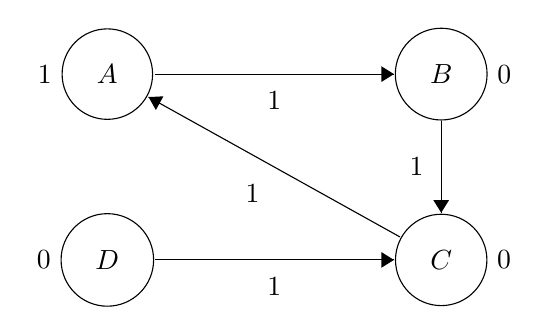
\begin{tikzpicture}[scale=0.2]
    \tikzset{lnode/.append style={inner sep=8pt,style={draw=black,circle}}}    
    \node[lnode,label=left:$1$] at (26.9,-27.1) {$A$};
    \node[lnode,label=right:$0$] at (48.1,-27.1) {$B$};
    \node[lnode,label=right:$0$] at (48.1,-38.9) {$C$};
    \node[lnode,label=left:$0$] at (26.9,-38.9) {$D$};
    \draw [black] (29.9,-27.1) -- (45.1,-27.1);
    \fill [black] (45.1,-27.1) -- (44.3,-26.6) -- (44.3,-27.6);
    \draw (37.5,-27.6) node [below] {1};
    \draw [black] (48.1,-30.1) -- (48.1,-35.9);
    \fill [black] (48.1,-35.9) -- (48.6,-35.1) -- (47.6,-35.1);
    \draw (47.6,-33) node [left] {1};
    \draw [black] (29.9,-38.9) -- (45.1,-38.9);
    \fill [black] (45.1,-38.9) -- (44.3,-38.4) -- (44.3,-39.4);
    \draw (37.5,-39.4) node [below] {1};
    \draw [black] (45.48,-37.44) -- (29.52,-28.56);
    \fill [black] (29.52,-28.56) -- (29.98,-29.38) -- (30.46,-28.51);
    \draw (36.12,-33.5) node [below] {1};
  \end{tikzpicture}
\end{center}
%
where, due to the fact that all the nodes have only one outgoing link, the edges
are labelled with 1s. Performing the first iteration we get
%
\begin{alignat*}{3}
  r_1(A) &= \sfrac{1}{2} \cdot (1\cdot0) + (1-\sfrac{1}{2}) &&= \sfrac{1}{2} \\
  r_1(B) &= \sfrac{1}{2} \cdot (1\cdot1)                    &&= \sfrac{1}{2} \\
  r_1(C) &= \sfrac{1}{2} \cdot (1\cdot0+1\cdot0)            && = 0 \\
  r_1(D) &= \sfrac{1}{2} \cdot 0                            &&= 0.
\end{alignat*}

We could continue with a second iteration
%
\begin{alignat*}{3}
  r_2(A) &= \sfrac{1}{2} \cdot (1\cdot0) + (1-\sfrac{1}{2}) &&= \sfrac{1}{2} \\
  r_2(B) &= \sfrac{1}{2} \cdot (1\cdot\sfrac{1}{2})         &&= \sfrac{1}{4} \\
  r_2(C) &= \sfrac{1}{2} \cdot (1\cdot\sfrac{1}{2}+0\cdot0) &&= \sfrac{1}{4} \\
  r_2(D) &= \sfrac{1}{2} \cdot 0                            && = 0, 
\end{alignat*}
%
and decide stop at the third one
%
\begin{alignat*}{3}
  r_3(A) &= \sfrac{1}{2} \cdot (1\cdot\sfrac{1}{4}) + (1-\sfrac{1}{2}) &&= \sfrac{5}{8} \\
  r_3(B) &= \sfrac{1}{2} \cdot (1\cdot\sfrac{1}{2})                    &&= \sfrac{1}{4} \\
  r_3(C) &= \sfrac{1}{2} \cdot (1\cdot\sfrac{1}{4}+0\cdot0)            &&= \sfrac{1}{8} \\
  r_3(D) &= \sfrac{1}{2} \cdot 0                                       &&= 0,
\end{alignat*}
%
which reveals that $B$ is the most similar node to $A$.